\documentclass[10pt]{article}

% Packages with options
\usepackage[english]{babel}
\usepackage[mathscr]{euscript}
\usepackage[margin=1in]{geometry} 
\usepackage[utf8]{inputenc}
\usepackage[small]{titlesec}

% Primary Packages
\usepackage{adjustbox, amsbsy, amsmath, amssymb, amsthm, bm, commath, chngcntr, dsfont, econometrics, fancyhdr, gensymb, graphicx, IEEEtrantools, longtable, marginnote, mathrsfs, mathtools, mdframed, natbib, parskip, pgf, setspace, subfigure, tabularx, textcomp, tikz}

% Hyperref Setup
\usepackage[pdfauthor={Manu Navjeevan},
			bookmarks=false,%
			pdftitle={Econ 425, Week 6},%
			pdftoolbar=false,%
			pdfmenubar=true]{hyperref} %hyperref needs to be last

% Rest of the setup is in the "Manu" package
\usepackage{manu}

%%%%%%%%%%%%%%%%%%%%%%%%%%%%%%%%%%%%%%%%%%%%%

\title{Econ 425, Week 6 \\ \large Neural Networks}%Title
\author{Manu Navjeevan}
\date{\today}

\begin{document}
\maketitle

\section{What is a Neural Network?}%
\label{sec:}

Neural Networks are probably what we think of when we think of Machine Learning. But philosophising over our brain's neural structure aside, what is a neural network?

A (feed-forward) neural network is really just a (relatively involved) parameteric model that we are going to try and fit using our data. In some ways we can think of it as a very complicated linear regression model. A typical neural network will have three main components, an \textit{input layer}, one or more (consecutive) \textit{hidden layers}, and finally an \textit{output layer}. Each layer will consist of one or more \textit{nodes} and the nodes will be connected to each other by \textit{edges}.
\begin{figure}[htb!]
	\centering
	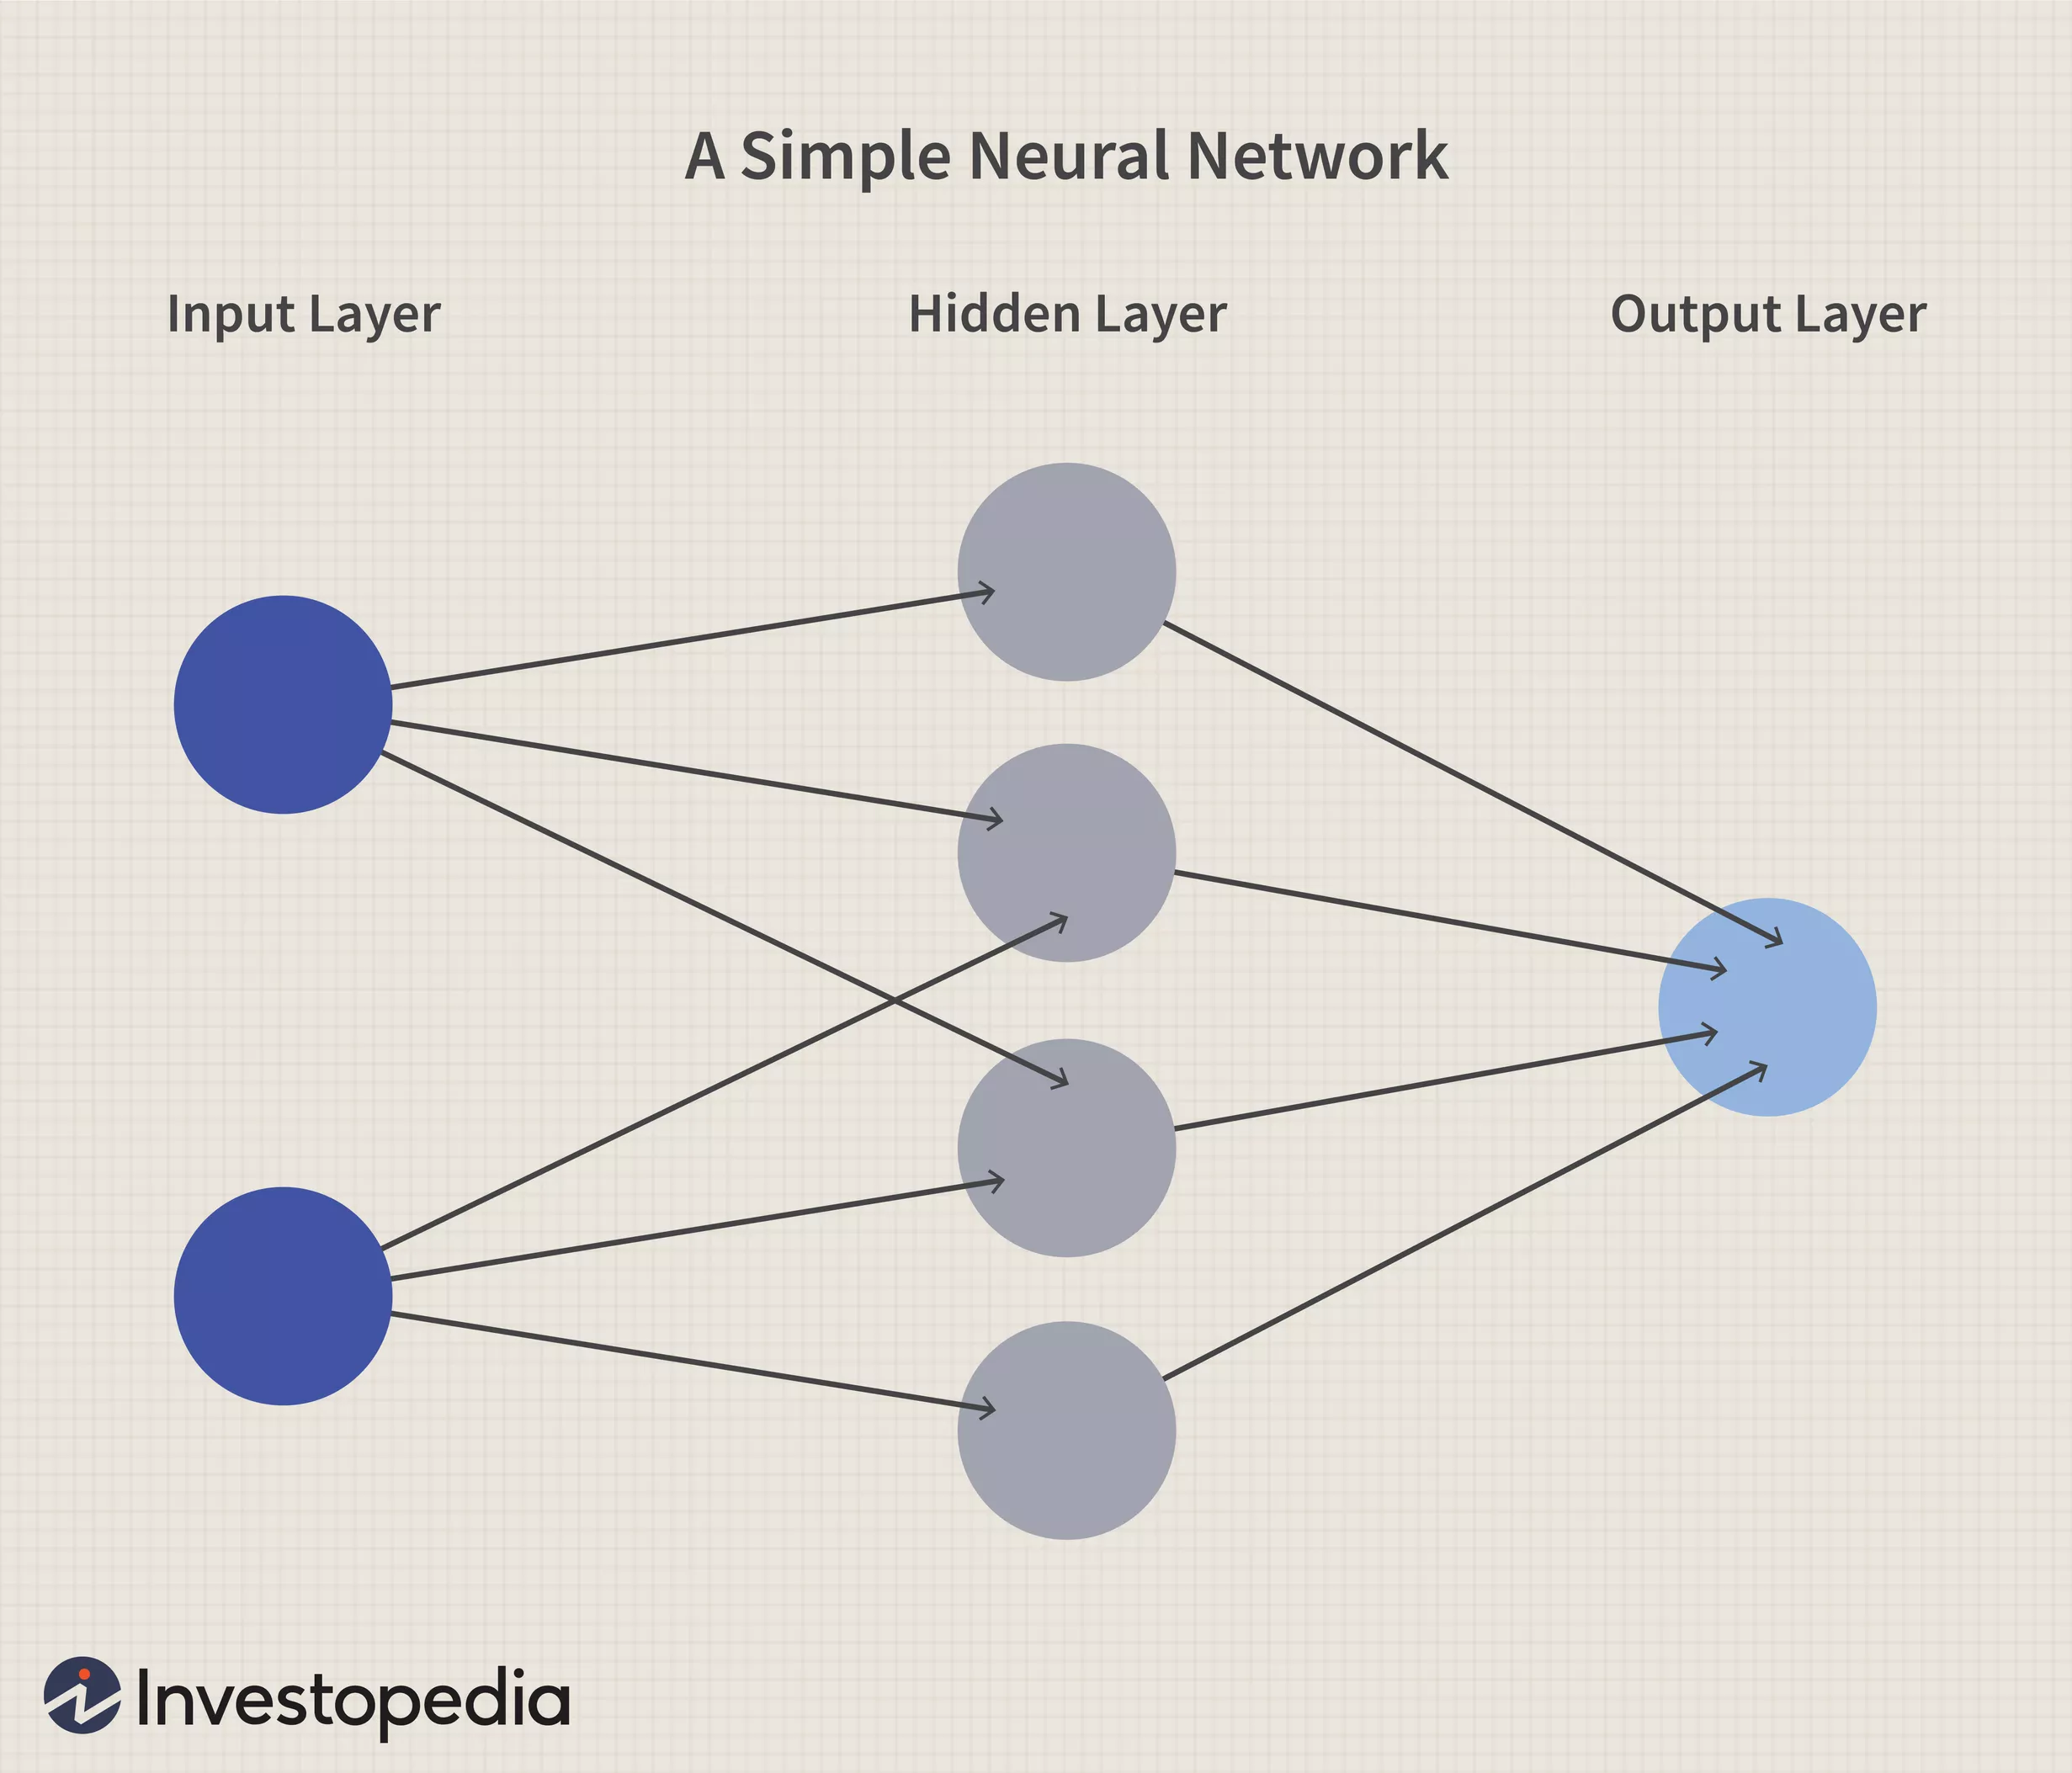
\includegraphics[width=0.7\linewidth]{neural-simple.png}
	\caption{A Simple Neural Network}%
	\label{fig:neural-simple}
\end{figure}

Note that edges are only between nodes in a prior layer to a node in a later layer. At each layer past the input layer each node will take in the outputs of the nodes that feed into it, take a linear combination of them, apply an activation function, and output into the next node (or just output if we are in the final output layer). 

To exemplify, consider the following neural network:

\begin{figure}[htb!]
	\centering
	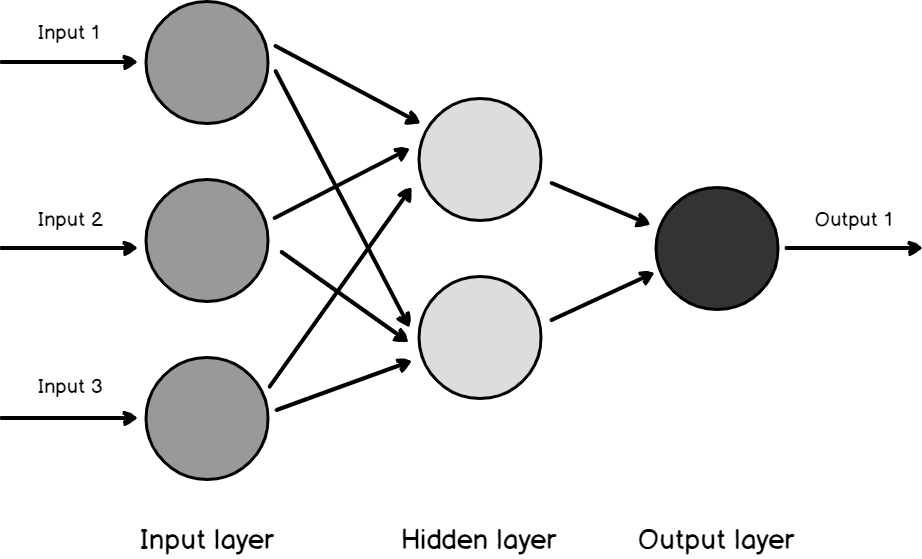
\includegraphics[width=0.7\linewidth]{neural-three.png}
	\caption{Another simple neural network}%
	\label{fig:neural-three}
\end{figure}

Let \(x_1\) denote input 1,  \(x_2\) denote input 2,  and \(x_3\) denote input 3. Consider the top node in the hidden layer (layer 2). This node is ``pointed to" or ``connected to" by all three nodes in the input layer. That means that it will take in \(x_1, x_2\) and  \(x_3\) and output something like:
 \[
	 \pi\left(\beta_0 + \beta_1x_1 + \beta_2x_2 + \beta_3x_3\right)
.\] 
where \(\pi\left(\cdot\right)\) is the ``activation function" that we will specify when we construct the neural network. When we initialize the neural net of course, we will not know the parameters \(\beta_0, \beta_1, \beta_2,\) and  \(\beta_3\). We will use our data to estimate these paramters (as well as the parameters on all the other nodes), which we will explain later.

This process of taking a linear combination of inputs, applying the activation function, and passing the output onto the next node happens layer by layer until we are at the final output layer. At this point, the same process of taking a linear combinations of inputs and applying an activation function. However the output is not passed on to another node. This output is simply considered the predicton of our model. When using our data to fit the model (or ``learn" the model), we will choose the parameters that minimize the distance between our prediction and the actual outcome of interest in the training data with respect to some cost function (least squares, log-cost, etc.).

A note on fitting. All together, the output function is very non-convex/complex in it's parameters. This means that there is definetly no closed form solution for the optimal parameter to choose and moreover that simple gradient descent is not garunteed to find a global optimum, even with relatively simple architecture and a straightforward cost function. This means that when fitting a neural net, we should start a few (maybe many) different starting points, run a gradient descent, and compare minimum across the various solutions you find. Computing the gradient is also not so straightforward and can become computationally involved for complex neural networks. All of this means that neural networks can be computationally invovled to fit and may take time to converge to an optimal solution.

\subsection{Activation Functions}

As we noted above, the activation function \(\pi(\cdot)\) that each node uses has to be specified. The various activation functions are given:
\begin{align*}
	\text{sigmoidal}: \pi(x) &= \frac{1}{1 + e^{-x}}\\
	\text{Leaky ReLU}: \pi(x) &= \max(0.1x,x) \\
	\tanh: \pi(x) &= \tanh(x) \\
	\text{Maxout}: \pi(x) &= \max(w_1x + b1, w_2x+b_2) \\
	\text{ReLU}: \pi(x) &= \max(0,x)\\
	\text{ELU}: \pi(x) &= \begin{cases}
		x & \text{if }x\geq 0 \\
		\alpha\left(\e^x-1\right)&\text{if }x<0
	\end{cases}	
\end{align*}
I am aware of theoretical results (very recent) regarding deep neural newtorks with sigmoidal and ReLU activation functions, but not for other activation functions. ReLU appears to be most commonly used. Note that the sigmoidal function is the same function we used in logistic regression.

\end{document}

